\chapter{Moving towards an online BCI system}
\label{ch:online_bci_system}


% ---------------------------------------------- 
% INTRODUCTION
% ---------------------------------------------- 
\section{Introduction}
\label{sec:online_bci_system_introduction}
% NOTE: "Introduction" exists in each chapter and gives a short intro to the chapter + what can be expected in the chapter

Whilst the focus of this master thesis is on the evaluation of offline \gls{mi} \gls{eeg} classification pipelines, this chapter aims to provide a link of these pipelines to a complete \gls{bci} system.
Some of the key differences in what is the wanted goal of a \gls{bci} system compared to that of a \gls{mi} \gls{eeg} classifier are discussed.
This includes the difference between classification and regression in the pipeline of a \gls{bci} system, working with relatively limited data and computational power and focusing on limiting risk rather than the best overall accuracy.
Next, some common steps in going from these proposed offline \gls{mi} \gls{eeg} classification pipelines to an online \gls{bci} are discussed.
Since these are provided as pointers rather than effective guidelines, most explanations in this chapter remain high-level.
This includes providing some details on working with continuous data, tricks to improve classification performance, the potential of spatial subsampling and a revision of smart mapping between predicted classes and the actions taken on the external device.


% ---------------------------------------------- 
% INTRODUCTION
% ---------------------------------------------- 
\section{BCI system try to solve another problem}
\label{sec:online_bci_system_different_goal}

\begin{figure}[t]
    \centering
    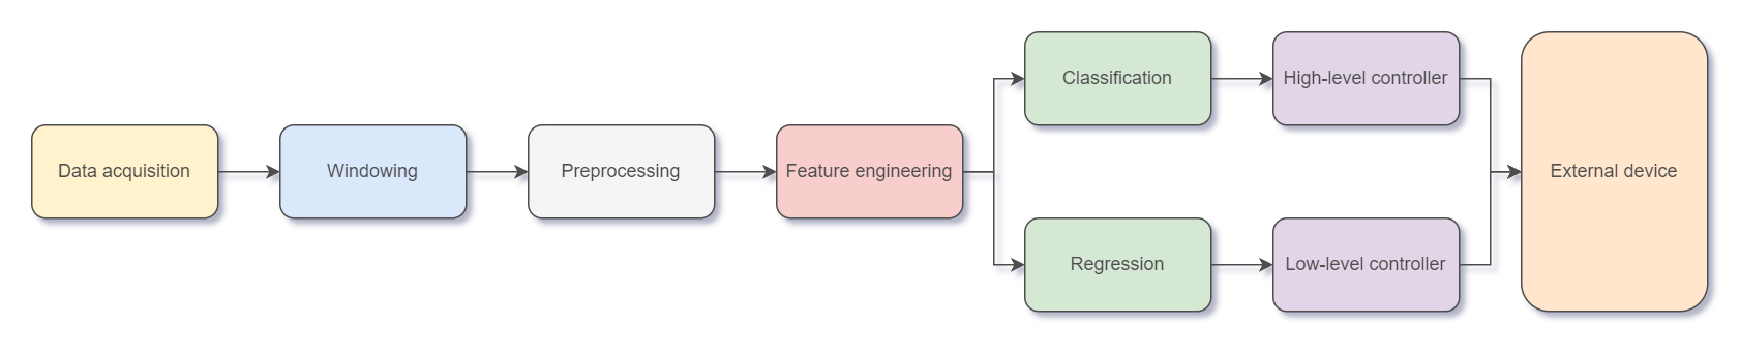
\includegraphics[width=\linewidth]{../images/online/bci_pipeline.pdf}
    \captionsetup{width=0.8\linewidth}
    \captionsetup{justification=centering}
    \caption{Overview of a complete BCI pipeline.}
    \label{fig:online_bci_system_full_bci_pipeline}
\end{figure}


Whilst the general pipeline for classifying brain signals discussed in Section \ref{sec:processing_signals_general_pipeline} forms the majority of the \gls{bci} system pipeline, the components to map predicted class labels to effective actions taken on the external device are missing.
Figure \ref{fig:online_bci_system_full_bci_pipeline} shows the complete \gls{bci} pipeline where a high-level controller for mapping classification labels to specific actions on the external device is present.
Whilst rather uncommon in \gls{bci} research, it is also possible for a regression model to be used to create a more low-level mapping to the external device \citep{bci_review_arnau}.
The difference between both approaches is discussed in the following section.
Some other differences are present, such as a far more complex dataset, relatively low-powered computational hardware and a focus on minimizing risk rather than maximising accuracy.
These things are also briefly discussed in the following sections.

% - - - - - - - - - -
% Classification vs regression
% - - - - - - - - - -

\subsection{Using classification vs regression in a BCI system}
\label{subsec:online_bci_system_different_goal_classi_vs_reg} 

As discussed in Section \ref{subsec:bci_common_use_cases_prosthesis_exoskeleton}, one of the use-cases for \glspl{bci} is their use as a novel interaction method for prosthesis and exoskeleton control.
Ideally, the control over such an exoskeleton would require some sort of continuous mapping rather than a discrete one.
A traditional exoskeleton might rely on muscle movement to create a near 1:1 mapping where continuous values are passed to the low-level controller which denotes the angles of the arm and as such the desired angles of the exoskeleton.
Regression algorithms can be used to map a feature vector, i.e. from \gls{emg}, to a continuous output that denotes such angles.

Since classification is discrete by design, such a near 1:1 mapping is not feasible.
Instead, an often limited amount of classes exist to keep learning possible and a high-level controller is used to map one class label with a relatively complex set of actions rather than just one minuscule one.
The design of such a system was already shown in Figure \ref{fig:example_arm_control} for a robot arm.
Intuitively, the mapping possible between a regressor and a low-level controller could be compared with the control of a joystick allowing fine control of movement in a game.
In that setting, classification linked to a high-level controller could be compared with the regular buttons on the game controller which are mapped to an action that performs multiple complex steps upon the press of one button.

An argument could be made that the regressor approach is more intuitive and allows for better control over the external device.
However, due to the discussed complexity of brain signals, creating an effective mapping from brain signals to a continuous value is a far harder problem than the classification of only a select few classes.
This is further illustrated by a lack of successful literature on proposed regression pipelines for \gls{eeg} systems as discussed by \citet{bci_review_arnau}.

% - - - - - - - - - -
% comp power
% - - - - - - - - - -

\subsection{Complexer data and less powerful systems}
\label{subsec:online_bci_system_different_goal_speed} 

The data used for the experiments of this master thesis, and most of the open-source \gls{mi} \gls{eeg} datasets available, contain data recorded in near lab-like environments.
Section \ref{sec:evaluation_data_source} discusses the used dataset for the experiments in this master thesis where it will become clear that these recordings are also relatively lab-like.
Whilst this makes for clean data, it is by no means representative of the real world.
As discussed in Section \ref{subsec:biomedical_signals_working_with_eeg_artefacts}, many artefacts such as electrode popping and \gls{emg} artefacts are expected when the \gls{bci} user is walking, talking or even just looking around.
This means the test metrics obtained from these-open source datasets are likely to be non-representative of their performance when used in a real-world setting.

Adding to this, the portability and affordability desired for a \gls{bci} system mean that the available hardware is often as cheap as possible, especially for the processing unit.
As such, complex deep learning models requiring specific \glspl{gpu} or drivers to be present are non-feasible for real-world use.
This causes a problem for the convolutional \gls{lstm} extension to EEGNet proposed in this master thesis, as is further discussed in Section \ref{sec:evaluation_pilot_studies} where some additional pilot studies are performed.

% - - - - - - - - - -
% risky errors
% - - - - - - - - - -

\subsection{Limiting risky errors}
\label{subsec:online_bci_system_different_goal_limit_risk} 

As discussed in Section \ref{sec:evaluation_eval_metrics}, reporting on test accuracy alone has little meaning for a \gls{bci} setting, where additional metrics such as the \gls{ppv} are desired to obtain a complete insight on the model's performance.
This is particularly important when moving to an online system.
A system having 80\% accuracy but where all misclassification results in the passive case being predicted, where no action is performed, is far more desirable than one with an accuracy of 90\% but where it performs a risky action 10\% of the time during misclassification.
Traditional optimisation of a model will typically only look at accuracy or loss metrics and as such doesn't take into account this information.
There exist multiple ways of calculating the risk-related metrics of a classifier.
For the evaluation of the pipelines in this master thesis, Section \ref{sec:evaluation_eval_metrics} details three such metrics that give insight into the risky behaviour of the classifier.

% ---------------------------------------------- 
% INTRODUCTION
% ---------------------------------------------- 
\section{Common steps towards an online BCI system}
\label{sec:online_bci_system_different_common_steps}

With the general difference between creating, training and optimizing a classifier and a complete \gls{bci} system discussed, some proposals are made on how to adopt the classification pipeline to consider these aspects.

% - - - - - - - - - -
% continuous data
% - - - - - - - - - -

\subsection{Working with continuous data}
\label{subsec:online_bci_system_different_common_steps_sliding_window} 

Due to the use of \gls{ers} and \gls{erd} potentials by using \gls{mi}, which can be induced without an external stimuli, there is no specific event onset (see section \ref{subsec:biomedical_signals_working_with_eeg_inducing_methods}).
As such, the windowing strategy used in the experiments of this master thesis is not applicable.
Whilst it could be made to work, by providing an event onset indication on regular time intervals when the user is allowed to perform a \gls{mi} task for classification, it is not the most attractive solution.
As such, sliding windows, preferably overlapping, should be used.
However, such a window design makes the problem complex to learn and classify.
As such, some of the evaluations discussed in Chapter \ref{ch:evaluation} should ideally be reproduced using such sliding windows to finetune parameters and gain insight into the model performance when using sliding windows.

% - - - - - - - - - -
% improving performance
% - - - - - - - - - -

\subsection{Improving classification performance and adding more classes}
\label{subsec:online_bci_system_different_common_steps_better_classi} 


Even when the classification results obtained are satisfactory, small risky errors can already be troublesome for some risky \gls{bci} systems.
As such, additional tricks should be put into place to increase the performance of these models w.r.t. risky misclassification.
For example, if using sliding windows and assuming that misclassification is independent of the previous sliding window, requiring three consecutive classifications of the same class before performing a specific action can reduce the original misclassification of that class from 20\% to just 0.8\% ($0.2*0.2*0.2$).
However, the assumption that misclassification is independent of the previous sliding window does not hold in real life, so the actual misclassification decrease will be less.
Alternatively, before performing a potentially risky action this action could be communicated to the user in such a way that the user can still cancel it.
This cancelling can then be done by some of the easier to detect \gls{emg} artefacts discussed in section \ref{subsec:biomedical_signals_working_with_eeg_artefacts} as these have high classification accuracy.
Another interesting technique is using the \gls{roc} curve for determining an ideal prediction threshold such that the FPR of risky actions is minimal as was discussed in Section \ref{subsubsec:processing_signals_evaluating_and_using_evaluation_valtest}.

% - - - - - - - - - -
% calibration
% - - - - - - - - - -

\subsection{Calibrating the classification pipeline before use}
\label{subsec:online_bci_system_different_common_steps_calibration} 

It was discussed that brain signals are non-stationary oscillatory signals that can vary greatly between subjects and even between sessions of the same subject.
Besides using techniques to reduce risky misclassification, it is often the case that calibration of a \gls{dl} model is performed.
The main idea behind calibration is using a data acquisition method for obtaining labelled samples of the subject wanting to use the \gls{bci} before actually trying to predict for that session of the subject.
These additional labelled samples are often obtained in less than 20 minutes \citep{eeg_model_eegnet}.
After being obtained, a previously trained model, either intersession or intersubject, is loaded and the additional data is fed to the model for further training.
The idea is that this reduces an intersubject or intersession problem to an intrasession problem, as the classifier has access to the data from the same session it asked to predict samples for after calibration.
Since this calibration data is often limited, a model can sometimes overfit the training data in such a small amount of time that the validation scores won't increase.
This often requires stopping certain parts of a model from learning, \textit{freezing} them, and only training the last part(s) of the model further on the additional data using a very low learning rate.

Calibration can have varying results, if too few samples are present and the model overfits right away neither validation nor test accuracy will increase and they often even decrease.
If too many new samples are present, it might be better to just train a completely new shallow model using an intrasession approach.
Finding the sweet spot is not an easy task and often it is too long in time for a user to enjoy the process of calibration each time they want to use the \gls{bci} system.
For these reasons, data augmentation techniques for \gls{eeg} are being proposed which aim to artificially increase the number of samples obtained from a short calibration period.
\citet{gan_eeg_augmentation} has shown the use of a \gls{gan} to augment such \gls{eeg} data with satisfactory results.



% - - - - - - - - - -
% spatial subsampling
% - - - - - - - - - -

\subsection{Spatial subsampling}
\label{subsec:online_bci_system_different_common_steps_subsampling} 

As discussed in section \ref{subsec:biomedical_signals_working_with_eeg_anatomy}, when it is known in which region of the brain the signals of interest are expected to originate, the channels can be subsampled to only include those that are of interest.
This decrease the complexity, making the prediction computationally easier to perform and thus easier to execute on the affordable and portable hardware desired from a general \gls{bci} system.
Additionally, removing the frontal electrodes will remove the channels most related to an artefact from facial muscle movement and eye movement.
This could help in reducing the added data complexity by removing some of the artefact-filled channels.

% - - - - - - - - - -
% mapping
% - - - - - - - - - -

\subsection{Configuring the high-level controller}
\label{subsec:online_bci_system_different_common_steps_mapping} 

Once the \gls{mi} \gls{eeg} pipelines are reconfigured to work better for the use of a sliding window in an online \gls{bci} setting, the mapping from classification labels to actions may be done.
Not only should this mapping take into account the \gls{ppv} of a class to determine which is most fit for taking risky actions, but the mapping and interaction with the external device itself should also be carefully designed to require the least possible steps to achieve the desired result.
This was already explained with the robotic arm example in Section \ref{subsec:bci_opportunities_obstacles_motivating_examples}.

Once an appropriate mapping is determined, implementing it such that the external device does the desired action can be a difficult task since many devices often have a different way of being programmatically controlled (interfacing method).
As discussed by \citet{bci_review_arnau}, there are currently proposals being made for standardized platforms such that multiple external devices such as exoskeleton and prosthesis share an equal interfacing method.
These standardized platforms can also allow for simulated interaction, which can be helpful when combined with \gls{vr} to let a new user test if a certain external device would work as desired. 

% ---------------------------------------------- 
% Other required changes
% ---------------------------------------------- 
\section{Chapter conclusions}
\label{sec:online_bci_system_other_changes_conclusion}

This chapter gave a brief overview of the challenges present when going from an offline \gls{mi} \gls{eeg} classification pipeline to an online \gls{bci} system.
Some broad steps were discussed that could be performed to facilitate this move to an online \gls{bci} system.
In the next chapter, some pilot studies are also discussed that provide initial results of some of the changes proposed in this section.
